\section{mo\-It\-Rand\-Next\-Move$<$ M $>$ Class Template Reference}
\label{classmo_it_rand_next_move}\index{moItRandNextMove@{moItRandNextMove}}
One of the possible {\bf mo\-Next\-Move}{\rm (p.\,\pageref{classmo_next_move})}.  


{\tt \#include $<$mo\-It\-Rand\-Next\-Move.h$>$}

Inheritance diagram for mo\-It\-Rand\-Next\-Move$<$ M $>$::\begin{figure}[H]
\begin{center}
\leavevmode
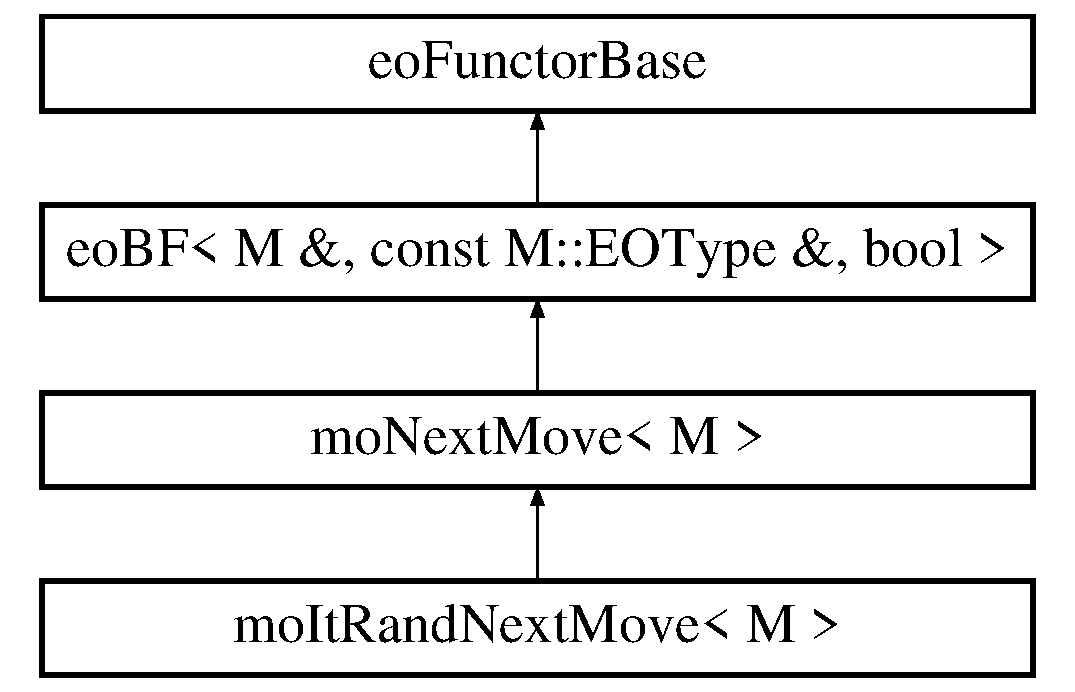
\includegraphics[height=4cm]{classmo_it_rand_next_move}
\end{center}
\end{figure}
\subsection*{Public Member Functions}
\begin{CompactItemize}
\item 
{\bf mo\-It\-Rand\-Next\-Move} ({\bf mo\-Rand\-Move}$<$ M $>$ \&\_\-random\_\-move\_\-generator, unsigned int \_\-iteration\_\-maximum\_\-number)
\begin{CompactList}\small\item\em The constructor. \item\end{CompactList}\item 
bool {\bf operator()} (M \&\_\-move, const {\bf EOT} \&\_\-solution)
\begin{CompactList}\small\item\em Generation of a new move. \item\end{CompactList}\end{CompactItemize}
\subsection*{Private Types}
\begin{CompactItemize}
\item 
typedef M::EOType {\bf EOT}\label{classmo_it_rand_next_move_y0}

\begin{CompactList}\small\item\em Alias for the type. \item\end{CompactList}\end{CompactItemize}
\subsection*{Private Attributes}
\begin{CompactItemize}
\item 
{\bf mo\-Rand\-Move}$<$ M $>$ \& {\bf random\_\-move\_\-generator}\label{classmo_it_rand_next_move_r0}

\begin{CompactList}\small\item\em A move generator (generally randomly). \item\end{CompactList}\item 
unsigned int {\bf iteration\_\-maximum\_\-number}\label{classmo_it_rand_next_move_r1}

\begin{CompactList}\small\item\em Iteration maximum number. \item\end{CompactList}\item 
unsigned int {\bf iteration\_\-number}\label{classmo_it_rand_next_move_r2}

\begin{CompactList}\small\item\em Iteration current number. \item\end{CompactList}\end{CompactItemize}


\subsection{Detailed Description}
\subsubsection*{template$<$class M$>$ class mo\-It\-Rand\-Next\-Move$<$ M $>$}

One of the possible {\bf mo\-Next\-Move}{\rm (p.\,\pageref{classmo_next_move})}. 

This class is a move ({\bf mo\-Move}{\rm (p.\,\pageref{classmo_move})}) generator with a bound for the maximum number of iterations. 



Definition at line 47 of file mo\-It\-Rand\-Next\-Move.h.

\subsection{Constructor \& Destructor Documentation}
\index{moItRandNextMove@{mo\-It\-Rand\-Next\-Move}!moItRandNextMove@{moItRandNextMove}}
\index{moItRandNextMove@{moItRandNextMove}!moItRandNextMove@{mo\-It\-Rand\-Next\-Move}}
\subsubsection{\setlength{\rightskip}{0pt plus 5cm}template$<$class M$>$ {\bf mo\-It\-Rand\-Next\-Move}$<$ M $>$::{\bf mo\-It\-Rand\-Next\-Move} ({\bf mo\-Rand\-Move}$<$ M $>$ \& {\em \_\-random\_\-move\_\-generator}, unsigned int {\em \_\-iteration\_\-maximum\_\-number})\hspace{0.3cm}{\tt  [inline]}}\label{classmo_it_rand_next_move_a0}


The constructor. 

Parameters only for initialising the attributes.

\begin{Desc}
\item[Parameters:]
\begin{description}
\item[{\em \_\-random\_\-move\_\-generator}]The random move generator. \item[{\em \_\-iteration\_\-maximum\_\-number}]The iteration maximum number. \end{description}
\end{Desc}


Definition at line 61 of file mo\-It\-Rand\-Next\-Move.h.

References mo\-It\-Rand\-Next\-Move$<$ M $>$::iteration\_\-maximum\_\-number, mo\-It\-Rand\-Next\-Move$<$ M $>$::iteration\_\-number, and mo\-It\-Rand\-Next\-Move$<$ M $>$::random\_\-move\_\-generator.

\subsection{Member Function Documentation}
\index{moItRandNextMove@{mo\-It\-Rand\-Next\-Move}!operator()@{operator()}}
\index{operator()@{operator()}!moItRandNextMove@{mo\-It\-Rand\-Next\-Move}}
\subsubsection{\setlength{\rightskip}{0pt plus 5cm}template$<$class M$>$ bool {\bf mo\-It\-Rand\-Next\-Move}$<$ M $>$::operator() (M \& {\em \_\-move}, const {\bf EOT} \& {\em \_\-solution})\hspace{0.3cm}{\tt  [inline]}}\label{classmo_it_rand_next_move_a1}


Generation of a new move. 

If the maximum number is not already reached, the current move is forgotten and remplaced by another one.

\begin{Desc}
\item[Parameters:]
\begin{description}
\item[{\em \_\-move}]the current move. \item[{\em \_\-solution}]the current solution. \end{description}
\end{Desc}
\begin{Desc}
\item[Returns:]false if the maximum number of iteration is reached, else true. \end{Desc}


Definition at line 73 of file mo\-It\-Rand\-Next\-Move.h.

References mo\-It\-Rand\-Next\-Move$<$ M $>$::EOT, mo\-It\-Rand\-Next\-Move$<$ M $>$::iteration\_\-number, and mo\-It\-Rand\-Next\-Move$<$ M $>$::random\_\-move\_\-generator.

The documentation for this class was generated from the following file:\begin{CompactItemize}
\item 
mo\-It\-Rand\-Next\-Move.h\end{CompactItemize}
